\documentclass{article}
\usepackage[a4paper]{geometry}
\usepackage{tikz}
\usetikzlibrary{trees}

\title{Elements of Language Processing and Learning\\
Lab assignment \\
Stage 1: Computing the Probability of a Tree\\
Report}
\author{Benno Kruit, 10576223\\Sara Veldhoen, 10545298}

\begin{document}
\maketitle

The objective is to compute the probability of a parse tree, e.g. a tree in the test set. 


In general, the probability of a tree is the product of the probabilities of the production rules that would have generated it.
This includes the the probabilities of the word leaves, which are lexical entries. This is illustrated in Figure 1.
We actually compute the log probability to avoid arithmetic underflow due to the multiplication of small probabilities. Therefore, in the algorithm we add together the log probabilites.

\begin{figure}
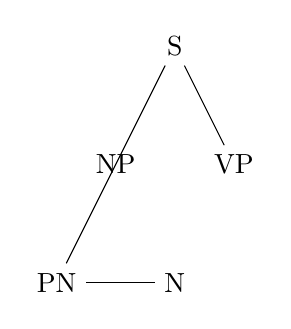
\begin{tikzpicture}

\node {S}
	child { node (left node) {NP}
		child {node (left node) {PN}}
		child {node (right node) {N}}
		}
	child {node (right node) {VP}}
    ;

\end{tikzpicture}
\caption{The probability of a tree is a multiplication of the probability of the production with the probability of its children}
\end{figure}

\paragraph{Implementation}
First, the tree is annotated. This binarizes the tree and creates nodes with names that correspond to the non-binarized structure. Then, we compute the log-probability of the annotated tree using the \texttt{logScoreHelper} function.

\paragraph{}
The function \texttt{logScoreHelper} essentially has two cases:
\begin{itemize}
	\item \textbf{Base case: preterminal node}\\
	 If the tree is a preterminal node, the child is a leaf with a terminal (a word). In this case, the lexicon is called to look up the probability of this production rule. If the lookup fails, it will return $\log(0)$, which is $-\infty$.
	\item \textbf{Recursive case: internal node}\\
	 If the tree is an inner node with trees as children, the grammar is called to look up  the probability of the production rule that produced this internal node. The probability of the children is computed via a recursive call to \texttt{logScoreHelper}. Here, a distinction is made between internal nodes with one or two children, thus calling the grammar for unary or binary rules respectively.

 The sum of the log of these probabilities is then returned. Similar to the base case, if the lookup fails,  it will return $\log(0)$, which is $-\infty$.
\end{itemize}

\paragraph{Results}
The log probability was computed on 10 trees from the test set.
For a few cases, the production rules or lexical items where never encountered in the training data, which resulted in a log probability of $-\infty$. For the rest, the log probabilities were in the range of $-100 < \log(p) < 0$.

\end{document}
